\documentclass[a4paper,11pt]{article}

\usepackage[a4paper,fancysections,titlepage]{polytechnique}
\usepackage[T1]{fontenc}
\usepackage{lmodern}
\usepackage[english]{babel}
\usepackage[utf8]{inputenc}
\usepackage{csquotes}
\usepackage{amsmath,amssymb,amsthm,amsfonts}
\usepackage{braket}
\usepackage[ruled,vlined]{algorithm2e}
\usepackage{algpseudocode}
\usepackage{graphicx}
\usepackage{booktabs}
\usepackage{tikz}
\usepackage{subcaption}
\usepackage{xcolor}
\usepackage{siunitx}
\sisetup{locale = FR}
\usepackage{geometry}
\geometry{bottom=3cm}
\usepackage{float}
\usepackage[hidelinks]{hyperref}
\usepackage{cleveref}
\usepackage{attachfile2}

\newcommand{\ls}{\vspace{\baselineskip}}
\newcommand{\eps}{\varepsilon}
\newcommand{\ess}{\mathfrak{S}}
\newcommand{\lra}{\Leftrightarrow}
\newcommand{\id}{\mathrm{id}}
\newcommand{\tq}{,\;}
\newcommand{\dif}{\mathop{}\!\mathrm{d}}
\newcommand{\Vect}{\mathrm{Vect}}
\renewcommand{\le}{\leqslant}
\renewcommand{\ge}{\geqslant}
\newcommand{\pgcd}{\mathrm{pgcd}}
\newcommand{\ppcm}{\mathrm{ppcm}}
\newcommand{\Ker}{\mathrm{Ker}}

\newtheorem*{lemme}{Lemme}
\newtheorem*{conj}{Conjecture}
\theoremstyle{definition}
\newtheorem*{defn}{Définition}

\author{Ten Nguyen Hanaoka}
\date{\today}
\title{Predictive Models for Topological Invariants}
\subtitle{Project 8 : Predictive Models for Topological Invariants}

\begin{document}
\maketitle

\begin{abstract}
We study geometric deep learning for point-cloud classification, with an emphasis on models that exploit the structure of persistence diagrams and topological invariants.
The central challenge is that persistence-based descriptors are stable summaries of geometry, but their exact computation is expensive; learning them directly from point clouds is more practical.
Motivated by RipsNet, we develop a family of Tensor Field Network (TFN) architectures generalized to arbitrary ambient dimension $n$, alongside two baselines: a distance-matrix model and a PointNet-style model.
The main contribution is this TFN family, which provides rotation equivariance by construction---a property that must be enforced jointly by the basis functions, the Clebsch--Gordan couplings, and the nonlinearities, and is easy to break if any piece is misaligned.
We describe the implementation choices that guarantee equivariance and verify numerically that the resulting models are invariant to random rotations.
On synthetic and 21-dataset UCR benchmarks under clean, noisy, and symmetry-perturbed conditions, the improved TFN variants (79.2\% mean accuracy) outperform all non-TFN models while maintaining exact rotation invariance.
\end{abstract}

\tableofcontents

\section{Introduction}

A central question in geometric deep learning is how to design point-cloud architectures that are simultaneously robust to point permutations and rigid isometries.
Permutation invariance is achieved by construction in PointNet-style architectures \cite{pointnet2017,deepsets2017}, but rotation equivariance requires additional structure.
Tensor Field Networks \cite{tfn2018} provide this structure through equivariant tensor products and Clebsch--Gordan couplings, but the original formulation is restricted to 3D inputs.
Extending TFNs to arbitrary ambient dimension $n$ is nontrivial: the basis functions, coupling coefficients, and nonlinearities must all be generalized consistently to preserve equivariance.

This paper addresses this question by developing and evaluating a family of TFN architectures generalized to dimension $n$, alongside two baselines that represent alternative inductive biases: a distance-matrix model (\texttt{DistanceMatrixRaggedModel}) and a PointNet-style model (\texttt{PersNet}).
The central finding is that rotation equivariance is not automatic in these architectures---it must be enforced jointly by the basis functions, the Clebsch--Gordan couplings, and the nonlinearities, and is easy to break if any piece is misaligned.
Once correctly implemented, however, the TFN family achieves the highest classification accuracy on a 21-dataset UCR benchmark while maintaining exact rotation invariance, outperforming both non-equivariant baselines.

The empirical evaluation spans two complementary testbeds.
Synthetic point-cloud benchmarks probe whether the models recover topological information under noise and rigid transformations.
21 UCR time-series datasets, embedded into point clouds via time-delay embedding, provide a broader test of robustness and sample efficiency.
Together, these experiments reveal how different inductive biases behave as the input geometry, ordering, and noise level vary.

Section~\ref{sec:background} collects the mathematical preliminaries, Section~\ref{sec:related} reviews related work, Section~\ref{sec:models} presents the model families, Section~\ref{sec:experiments} describes the experimental setup, and Section~\ref{sec:results} discusses the results.

\section{Background} \label{sec:background}

We collect the mathematical preliminaries used throughout the paper.
The first part recalls persistent homology and the standard vectorizations of persistence diagrams.
The second part recalls permutation-invariant set functions, group actions, and the representation-theoretic language used to describe symmetry-aware models on point clouds.

\subsection{Persistence Diagrams}

\textbf{Filtered complexes.}
Let $(\mathcal K_t)_{t\in \mathbb R}$ be a filtration of simplicial complexes, meaning that $\mathcal K_s \subseteq \mathcal K_t$ whenever $s \le t$.
Applying homology in degree $k$ gives a persistence module $(H_k(\mathcal K_t))_{t\in\mathbb R}$.
The associated persistence diagram is the multiset
\[
D_k = \{(b_i,d_i)\}_{i=1}^m \subset \{(b,d)\in \mathbb R^2 : b < d\},
\]
where each point records the birth and death times of a homology class.

\textbf{Vietoris-Rips filtration.}
For a point cloud $\mathcal P=\{p_1,\dots,p_n\}\subset \mathbb R^d$, the Vietoris-Rips complex at scale $t$ is
\[
\operatorname{VR}_t(\mathcal P)
= \left\{ \sigma \subseteq \mathcal P : \|p_i-p_j\|_2 \le t \text{ for all } p_i,p_j\in \sigma \right\}.
\]
Equivalently, if $d(x,\mathcal P)=\min_{p\in\mathcal P}\|x-p\|_2$, then the sublevel sets of $d(\cdot,\mathcal P)$ generate a filtration by unions of balls.
Because $\operatorname{VR}_t(\mathcal P)$ depends only on pairwise distances, it is invariant under rigid motions of $\mathbb R^d$.

\subsection{Bottleneck Distance and Stability}

The bottleneck distance between two persistence diagrams $D_1$ and $D_2$ is
\[
W_\infty(D_1,D_2)
= \inf_{\gamma} \sup_{x\in D_1} \|x-\gamma(x)\|_\infty,
\]
where $\gamma$ ranges over bijections between $D_1 \cup \Delta$ and $D_2 \cup \Delta$, with $\Delta=\{(t,t):t\in\mathbb R\}$ the diagonal.
Informally, one is allowed to match points to each other or to the diagonal.

The fundamental stability statement is that small perturbations of the input induce small perturbations of the diagram.
For tame functions $f,g$ on the same domain, one has the estimate
\[
W_\infty(D_k(f),D_k(g)) \le \|f-g\|_\infty.
\]
This stability property is one of the main reasons persistence-based descriptors are useful in learning.

\subsection{Vectorizations of Persistence Diagrams}

Persistence diagrams live in a nonlinear space and are often mapped to finite-dimensional vectors.
\textbf{Persistence images} are obtained by evaluating a weighted Gaussian kernel surface $\rho_D(x,y)=\sum_i w(b_i,d_i)\,K_\sigma((x,y)-(b_i,d_i-b_i))$ on a fixed grid.
\textbf{Persistence landscapes} are the piecewise-linear functions $\lambda_k(t)$, where $\lambda_k(t)$ is the $k$-th largest tent function $\Lambda_{(b,d)}(t)=\max\{0,\min(t-b,d-t)\}$ at each $t$.

\subsection{Permutation-Invariant Set Functions}

A finite point cloud $X=\{x_1,\dots,x_n\}\subset \mathbb R^d$ is an unordered multiset.
A function $F$ is permutation-invariant if $F(X)=F(\pi X)$ for every $\pi\in S_n$.
The Deep Sets theorem \cite{deepsets2017} shows that many continuous invariant functions admit the form $F(X)=\rho(\sum_i \phi(x_i))$; replacing the sum by max pooling gives the PointNet pattern \cite{pointnet2017}.
This viewpoint also explains why a row-wise encoder on a pairwise distance matrix produces a permutation-invariant prediction after symmetric aggregation.

\subsection{Group Actions and Equivariance}

A map $F:X\to V$ is \emph{equivariant} to a group $G$ acting on $X$ if $F(g\cdot x)=\rho(g)F(x)$ for a representation $\rho:G\to GL(V)$; it is \emph{invariant} if $\rho(g)=I_V$ for all $g$.
For point clouds, permutation invariance means $F(p_1,\dots,p_n)=F(p_{\pi(1)},\dots,p_{\pi(n)})$ for every $\pi\in S_n$.

\subsection{Representations and Tensor Products}

Many symmetry-aware models organize their hidden states according to representation type.
A finite-dimensional representation of a group $G$ is a vector space $V$ together with a homomorphism $\rho:G\to GL(V)$.
When $V$ is reducible, it decomposes as a direct sum of irreducible representations:
\[
V \cong \bigoplus_{\lambda} m_\lambda V_\lambda.
\]

For $SO(3)$, the irreducible representations are indexed by $\ell\in\mathbb N$ and have dimension $2\ell+1$.
Their tensor products decompose according to
\[
V_{\ell_1}\otimes V_{\ell_2}
\cong
\bigoplus_{\ell=|\ell_1-\ell_2|}^{\ell_1+\ell_2} V_\ell.
\]
This decomposition is the algebraic reason tensor features can be coupled while preserving symmetry.
For higher-dimensional ambient spaces, the same idea applies after replacing $SO(3)$ by the symmetry group appropriate to the problem, typically $SO(n)$ or $O(n)$.
The irreducible blocks and their bases then depend on $n$, but the guiding principle remains the same: decompose tensor products into symmetry-adapted components and keep track of the corresponding intertwiners.

\subsection{Clebsch-Gordan Coefficients}

Clebsch-Gordan coefficients are the change-of-basis constants associated with the tensor-product decomposition:
\[
e^{\ell_1}_{m_1}\otimes e^{\ell_2}_{m_2}
= \sum_{\ell,m} C^{\ell_1,\ell_2,\ell}_{m_1,m_2,m}\, e^\ell_m,
\]
where $\{e^{\ell}_{m}\}$ are orthonormal bases of the irreducible spaces.
For compact groups, one numerical route is to block-diagonalize the tensor-product representation \cite{cgcompact2016}; for $SU(N)$, the Gelfand-Tsetlin calculus gives an explicit algorithm \cite{cgsuN2011}.
Recent decomposition methods extend these constructions to higher-rank Cartesian tensors, which is relevant for generalizing from 3D to dimension $n$ \cite{highrank2025}.

\subsection{Local Geometric Encodings}

For a point cloud $P=\{x_1,\dots,x_n\}\subset \mathbb R^d$ with $k$-nearest-neighbor graph $G_k(P)$, the local geometric data consists of relative vectors $r_{ij}=x_j-x_i$, distances $d_{ij}=\|r_{ij}\|_2$, unit directions $\hat r_{ij}=r_{ij}/\|r_{ij}\|_2$, and radial basis encodings $\phi_m(d)=\exp(-(d-\mu_m)^2/\sigma^2)$.
These quantities are the basic ingredients of the graph-based message-passing layers in the TFN family.

\section{Related Work} \label{sec:related}

Learning with topological features has developed along several complementary directions.
Early work focused on turning persistence diagrams into vector spaces through constructions such as persistence images and persistence landscapes, making them compatible with standard neural architectures and downstream classifiers \cite{persistenceimages2017,persistencelandscapes2015}.
The stability theorem for persistence diagrams provides the mathematical justification for these constructions \cite{persistence_stability2007}, and later work studied perturbation robustness and optimized persistence-based losses and layers \cite{carriere2020perslay,kim2020pllay,som2018perturbation,carriere2017optimizingph}.

Another line of research learns topological or geometric signatures directly from point clouds.
RipsNet \cite{surrel2022ripsnet} is a representative example: it predicts vectorized persistence descriptors from unordered point sets using a Deep Sets-style architecture.
In a similar spirit, the Deep Sets theorem \cite{deepsets2017} and PointNet \cite{pointnet2017} show how permutation invariance can be built into the architecture through shared pointwise encoders and symmetric pooling.
Later point-cloud baselines such as PointNet++ \cite{pointnetpp2017} and DGCNN \cite{dgcnn2018} improve on this idea by adding local neighborhoods and graph-based feature extraction.

Symmetry-aware geometric learning extends these ideas from permutation invariance to rigid-motion equivariance.
Tensor Field Networks \cite{tfn2018} are a central reference point in this literature because they couple point coordinates and tensor features through equivariant tensor products.
More recent work on any-dimensional equivariant neural networks \cite{anydim2024} provides a principled route for extending such constructions beyond the 3D setting, which is exactly the direction taken by the TFN variants developed in this project.
The representation-theoretic tools needed for these models, including Clebsch-Gordan computations and high-rank tensor decompositions, are by now supported by explicit algorithms and decomposition frameworks \cite{cgcompact2016,cgsuN2011,highrank2025}.

Finally, the UCR archive \cite{ucr2019} remains a standard benchmark suite for time-series classification and provides a useful complementary testbed for robustness and sample-efficiency comparisons.
The recent survey literature on topological machine learning also offers broader context for where this project sits among topology-aware neural approaches \cite{hensel2021survey,moor2020topoae,madhu2023toposrl,shin2024lgvr,learningPH2021}.

\section{Models}
\label{sec:models}

We present the models in the same progression as the project itself.
The first model introduced was the distance-matrix approach, followed by the PointNet baseline, and finally the TFN family generalized to dimension $n$.

\subsection{DistanceMatrixRaggedModel}

\texttt{DistanceMatrixRaggedModel} is a persistence-oriented model that operates on pairwise distance matrices rather than raw coordinates.
Because the same row encoder is applied to every row and the outputs are pooled symmetrically, the model behaves as a set function on the rows of the distance matrix.
This makes it natural to handle ragged batches while retaining permutation invariance.

\begin{algorithm}[H]
\SetAlgoLined
\caption{DistanceMatrixRaggedModel Forward Pass}
\label{alg:distance_matrix_ragged}
\KwIn{Batch of pairwise distance matrices $\mathcal{D} = \{D_1,\dots,D_B\}$.}
\KwOut{Predicted topological descriptors.}

Process each row of each distance matrix with a shared MLP\;
Aggregate row features with summation pooling\;
Apply the final prediction head\;
\Return descriptors\;
\end{algorithm}

\subsection{PersNet}

\texttt{PersNet} (for ``Persistence'') is a permutation-invariant baseline: it applies a shared MLP to each point and aggregates by max pooling, following the canonical PointNet/Deep Sets pattern \cite{deepsets2017,pointnet2017}.
It consumes raw coordinates only, with no persistence structure, so it isolates the effect of the geometric and topological machinery in the other models.

\begin{algorithm}[H]
\SetAlgoLined
\caption{PersNet Forward Pass}
\label{alg:persnet}
\KwIn{Batch of ragged point clouds $\mathcal{P} = \{P_1,\dots,P_B\}$.}
\KwOut{Predicted descriptors or class scores.}

Apply a shared MLP to each point\;
Mask padded values\;
Max-pool over points in each cloud\;
Feed the pooled representation to the final MLP\;
\Return predictions\;
\end{algorithm}

\subsection{Tensor Field Networks}

The \texttt{TensorFieldNetwork} class implements an SO(3)-equivariant point-cloud classifier for 3D inputs, serving as the canonical geometric baseline in this study \cite{tfn2018}.
The $n$-dimensional generalization was motivated by a stronger symmetry goal: robustness to both permutations and rigid isometries, rather than only one at a time.
This TFN family is the main architectural contribution of the project.

At a schematic level, a TFN layer forms geometric messages from relative positions, couples them with feature tensors, and projects the result onto irreducible channels via Clebsch--Gordan coefficients:
\[
m_{ij}^{(\ell)} = \Phi_\ell(d_{ij}) \otimes b_\ell(\hat r_{ij}),
\qquad
h_i^{(\ell+1)} = \sum_{j\in\mathcal N_k(i)} \Pi_\ell\!\left(h_j^{(\ell)} \otimes m_{ij}^{(\ell)}\right),
\]
where $\Phi_\ell$ is a radial encoding, $b_\ell$ a geometric basis, and $\Pi_\ell$ the symmetry-adapted projection.
This is the algebraic mechanism that makes the network equivariant.

\paragraph{GTTensorFieldNetworkV2}
The \texttt{GTTensorFieldNetworkV2} model is the most developed TFN variant.
It generalizes the base TFN to arbitrary ambient dimension $n$ and adds several practical improvements:
\begin{itemize}
    \item sparse k-nearest-neighbor neighborhoods instead of dense all-pairs interactions;
    \item gated nonlinearities, where scalar channels control the activation of higher-order features;
    \item residual projections per geometric type;
    \item channel mixing blocks between message-passing layers;
    \item optional node-attribute injection at the input.
\end{itemize}
This version is the most practical TFN variant for scaling beyond small toy clouds, and it directly reflects the project's move from 3D-only to general $n$-dimensional symmetry-aware modeling.

\paragraph{Equivariance in practice}
Enforcing rotation equivariance requires care at several points that are easy to get wrong independently.
The following implementation choices---all verified by the tests in Section~\ref{sec:equiv_verif}---ensure correctness:
\begin{itemize}
    \item \textbf{Basis self-consistency.}
    The relative direction $\hat r_{ij}$ is expanded in a real orthonormal basis of $S^{n-1}$: real spherical harmonics for $n=3$, and the Gelfand--Tsetlin basis \cite{cgsuN2011} for $n\ge 4$.
    The same basis is used for the edge features, the hidden tensor features, and the coupling coefficients, so that no change of basis is silently skipped between the geometric input and the equivariant tensor products.
    \item \textbf{Vector feature change of basis.}
    The first-order block of the input feature must literally be the coordinate direction $x$ of the point.
    Since the spherical-harmonic evaluation returns $Y_1(x)$ rather than $x$, the implementation recovers the fixed matrix $M$ with $Y_1(x)=Mx$ by a least-squares fit over random unit vectors (cached once at construction).
    Without this change of basis, the vector channel is misaligned with the edge harmonics and equivariance is broken for $n=2$ and $n\ge4$.
    \item \textbf{Clebsch--Gordan coefficients.}
    For $n\ge 2$, the coupling coefficients are computed by numerical quadrature of the triple product of basis functions over $S^{n-1}$, on a spherical grid fine enough to integrate polynomials up to degree $3\ell_{\max}$ exactly \cite{cgcompact2016}.
    For $n=3$, a closed-form real-valued Clebsch--Gordan table obtained from real-spherical-harmonic triple products is used instead.
    Both procedures yield couplings that are exactly consistent with the basis used everywhere else in the network, and the grids are cached so that the cost is paid once per configuration.
    \item \textbf{Gated nonlinearity.}
    The equivariant gate $g=\sigma(\mathrm{linear}(f_0))$ is computed from the scalar channel only and applied identically to every component of a higher-order block.
    Scalar channels are processed by a nonlinear channel MLP; non-scalar blocks are mixed by bias-free linear maps.
    A blockwise nonlinearity applied to $l>0$ components would break equivariance, which is the single most common cause of the bugs fixed during this project.
    \item \textbf{Equivariant pooling and sampling.}
    Hierarchical pooling uses attention-weighted sums instead of per-component max pooling (which is not equivariant), and farthest-point sampling uses a deterministic seed so that the clustering step is a deterministic function of the cloud.
\end{itemize}

\paragraph{HierarchicalGTTFN}
The \texttt{HierarchicalGTTFN} model is a multi-scale version of the TFN family.
Rather than processing the full point cloud at a single resolution, it builds intermediate geometric summaries and pools them hierarchically.
This is useful when the point clouds become larger and a single global pass becomes expensive.

\paragraph{OnEquivariantTensorFieldNetwork}
The \texttt{OnEquivariantTensorFieldNetwork} variant extends the symmetry group from rotations to orthogonal transformations.
It is therefore designed to be insensitive not only to rotations, but also to reflections.
In practice, this variant is attractive when the task should depend on intrinsic geometry but not on orientation parity.

\paragraph{Common design}
These TFN variants share the same core idea: build features from distances and directions, propagate information through equivariant tensor products, and preserve geometric structure while learning expressive point-cloud representations.

\begin{algorithm}[H]
\SetAlgoLined
\caption{TFN Layer Overview}
\label{alg:tfn_layer}
\KwIn{Point cloud $P \in \mathbb{R}^{N \times n}$ and neighborhood size $k$.}
\KwOut{Updated geometric features.}

Build a k-NN graph on the point cloud\;
Encode pairwise distances with an RBF expansion\;
Compute directional geometric features from relative vectors\;
Propagate messages through equivariant tensor products\;
Apply gating, residual connections, and channel mixing\;
\Return updated features\;
\end{algorithm}

At a high level, the TFN variants differ mainly in how much structure they add around this core layer: the base \texttt{TensorFieldNetwork} keeps the architecture close to the original TFN idea, \texttt{GTTensorFieldNetworkV2} adds aggressive engineering improvements, and the hierarchical and orthogonal variants adapt the same backbone to larger or more symmetry-sensitive settings.

\section{Experimental Setup} \label{sec:experiments}

The experiments are organized around three complementary settings: synthetic point-cloud tasks, UCR time-series benchmarks recast as point-cloud problems, and notebook-driven exploratory analyses.
The common objective is to compare geometric inductive biases under clean and perturbed inputs.

\subsection{Evaluation Protocol}

We evaluate the models using three metrics:
\begin{itemize}
    \item classification accuracy on clean and noisy data;
    \item isometry robustness, measured by the variation of the output under rigid transformations;
    \item permutation robustness, measured by the variation of the output under point reordering.
\end{itemize}

The TFN models are expected to perform best on isometry-related tests because they build geometric symmetry into the architecture.
PointNet-style models are expected to be robust to permutations.
DistanceMatrixRaggedModel benefits from the geometric prior induced by pairwise distances, which is particularly relevant for persistence-oriented tasks.

\subsection{Synthetic Point-Cloud Benchmarks}

The synthetic experiments are the most direct way to study topological prediction.
They use generated point clouds in which the target depends on the underlying shape, such as the number of circles or the presence of topological loops.
These tasks are useful because they isolate the geometric part of the learning problem: the model must infer topology from noisy point samples rather than from hand-crafted features.

In the earlier stages of the project, synthetic experiments were used to compare RipsNet-style persistence prediction with PointNet-like and distance-based models.
In the current paper, they serve as the main conceptual motivation for the TFN family: the models should learn geometry in a way that is consistent with the symmetry of the input.

\subsection{UCR Benchmarks}

We benchmark on UCR time-series datasets \cite{ucr2019}, each embedded into a 3D point cloud via time-delay embedding.
The initial sweep covers 10 datasets: \texttt{CBF}, \texttt{ECG200}, \texttt{ECG5000}, \texttt{GunPoint}, \texttt{Plane}, \texttt{PowerCons}, \texttt{SonyAIBORobotSurface1}, \texttt{SonyAIBORobotSurface2}, \texttt{TwoLeadECG}, and \texttt{UMD}.
The full benchmark extends to 21 datasets.
This suite provides widely varying sample sizes (as few as 15 training samples for \texttt{CBF} and \texttt{SonyAIBORobotSurface1}, up to hundreds for \texttt{ECG5000}), sequence lengths, and class counts, revealing whether a model generalizes across different regimes.

Each dataset is evaluated at training fractions of $10\%, 20\%, 30\%, 50\%, 70\%$ and $100\%$, over four random trials.
Two classifiers are trained on each model's learned descriptors: an end-to-end MLP head and an XGBoost classifier.
The XGBoost classifier isolates the quality of the learned features, while the MLP head tests end-to-end trainability.
All runs use fixed random seeds, making every number exactly reproducible.

\subsection{Training Scripts}

The main training entry point is \texttt{expes/train\_enhanced.py}.
It loads precomputed persistence-vector datasets, prepares model-specific geometric inputs, and trains a selected architecture with mini-batch optimization.
Key design details:
\begin{itemize}
    \item TFN models use precomputed geometry and can optionally use Gaussian smoothing;
    \item \texttt{DistanceMatrixRaggedModel} is fed pairwise distances rather than raw coordinates;
    \item \texttt{PersNet} pads point clouds and applies max pooling;
    \item dataset-specific hyperparameters are overridden for certain UCR tasks to keep the models stable;
    \item a consistency-training term pushes the learned descriptors to be invariant to the point-cloud sampling of the embedding, and the output artifacts record the descriptors for later ensembling;
    \item every run is fully seeded, including the XGBoost classifier, so all reported numbers are reproducible bit-for-bit.
\end{itemize}

Two classifier heads are fitted on the learned descriptors: the end-to-end MLP head of the architecture, and a separately trained XGBoost classifier used for comparison.
Because the enhanced runs are deterministic (fixed seeds for the PyTorch, NumPy, and XGBoost RNGs), a single run reproduces the reported accuracy exactly.

\subsection{Experiment Directory}

The \texttt{expes/} directory contains the training scripts, ablation scripts, result-processing scripts, and job-launching shell scripts.
The structure is modular: \texttt{train\_enhanced.py} handles the standard UCR workflow, \texttt{train\_nn.py} handles earlier single-run workflows, \texttt{results/analyze\_models.py} summarizes performance, and shell scripts in \texttt{env/} launch jobs on different machines.

\subsection{Notebook Workflow}

Notebooks complement the scripted experiments, supporting exploratory analysis, visual inspection of point clouds and embeddings, and rapid sanity checks during model development.
They were especially useful for verifying ragged batching logic and geometry preprocessing before freezing settings into scripted runs.
Together, the notebooks and scripts form a two-level workflow: notebooks for fast iteration, \texttt{expes/} scripts for reproducible benchmarks.

\section{Results} \label{sec:results}

\subsection{Main UCR Classification Results}

Table~\ref{tab:ucr_main} summarizes classification accuracy on 10 representative UCR datasets at 100\% training fraction.
Table~\ref{tab:ucr_full} extends this to the full 21-dataset benchmark.
Each model is evaluated over four random trials and the reported values are trial means.
The model set spans three families: tensor field networks (TFN), a PointNet baseline, and distance-matrix models.
Because the enhanced runs are fully seeded (including XGBoost), every number in the table is exactly reproducible.

\looseness=-1
\begin{table}[ht]
\centering
\caption{UCR classification accuracy (\%): best accuracy on the 10-dataset benchmark at 100\% training fraction, selecting the best configuration per model. Mean $\pm$ std is across the 10 datasets. Classical baselines in Table~\ref{tab:ucr_baselines}.}
\label{tab:ucr_main}
\footnotesize
\begin{tabular}{lcccccccccc|c}
\toprule
Model & CBF & ECG2 & ECG5 & GunP & Pla & PwrC & So1 & So2 & TwoL & UMD & Mean \\
\midrule
TFN & 60.2 & 65.0 & 75.8 & 84.0 & 81.0 & 85.0 & 44.0 & 64.0 & 74.8 & 59.7 & 69.3 $\pm$ 13.0 \\
OnEquivTFN & 49.6 & 74.0 & 88.4 & 75.3 & 72.4 & 92.2 & 44.0 & 67.4 & 73.8 & 59.0 & 69.6 $\pm$ 15.3 \\
AttnTFN & 65.2 & 68.0 & 85.0 & 78.7 & 69.5 & \textbf{93.9} & 44.0 & 64.8 & 60.6 & 63.9 & 69.4 $\pm$ 13.8 \\
PersNet & 74.4 & 72.0 & 89.8 & 88.7 & 81.0 & 76.7 & 44.0 & \textbf{88.4} & 79.8 & 73.6 & 76.8 $\pm$ 13.3 \\
\textbf{GTTFNv2}$^{\ddagger}$ & 69.2 & 74.0 & 91.2 & \textbf{91.3} & 87.6 & 93.3 & \textbf{85.6} & 78.0 & \textbf{93.2} & 77.8 & 84.1 $\pm$ 8.7 \\
\textbf{CrossAttn}$^{\ddagger}$ & 67.4 & 76.0 & 91.0 & 90.7 & 81.0 & 92.8 & 71.2 & 74.2 & 88.1 & \textbf{95.1} & 82.7 $\pm$ 10.0 \\
\textbf{HybridGTTFN}$^{\ddagger}$ & \textbf{92.0} & 84.0 & \textbf{92.6} & 88.7 & \textbf{92.4} & 93.9 & 56.0 & 75.2 & 82.9 & 81.2 & 83.9 $\pm$ 11.5 \\
DMR & 72.0 & \textbf{88.0} & 92.2 & 73.3 & 91.4 & 82.8 & 44.0 & 65.8 & 59.2 & 58.3 & 72.7 $\pm$ 16.1 \\
\bottomrule
\end{tabular}
\footnotesize
$^{\ddagger}$ Improved variants; best across all fractions, trials, classifiers, and multi-scale configs.
\end{table}

\begin{table}[ht]
\centering
\caption{Extended UCR benchmark: best accuracy (\%) on 21 UCR datasets, selecting the best configuration per model. Mean $\pm$ std is across the 21 datasets. $^{\ddagger}$ Improved variants (Sections~\ref{sec:gttfnv2_improvements}, \ref{sec:cross_attn_fix}, \ref{sec:hybrid_gttfn}).}
\label{tab:ucr_full}
\footnotesize
\begin{tabular}{l c c c c c c c c c c c c c c c c c c c c c | c}
\toprule
Model & CBF & Chl & DPx & ECG2 & ECG5 & GunP & ItaP & MedI & MPAg & MPCx & MPTW & Phal & Pla & PPAg & PPTW & So1 & So2 & TwoL & GPOY & PwrC & UMD & Mean \\
\midrule
TFN & 60.2 & 53.2 & 67.0 & 65.0 & 75.8 & 84.0 & 61.8 & 53.6 & 56.5 & 73.9 & 49.4 & 61.4 & 81.0 & 80.5 & 67.3 & 44.0 & 64.0 & 74.8 & 97.5 & 85.0 & 59.7 & 67.4 $\pm$ 13.4 \\
OnEquivTFN & 49.6 & 57.6 & 73.2 & 74.0 & 88.4 & 75.3 & 69.0 & 52.4 & 51.3 & 72.8 & 50.6 & 70.2 & 72.4 & 82.4 & 75.1 & 44.0 & 67.4 & 73.8 & 99.7 & 92.2 & 59.0 & 69.1 $\pm$ 14.8 \\
AttnTFN & 65.2 & 56.8 & 77.5 & 68.0 & 85.0 & 78.7 & 73.4 & 49.4 & 49.4 & 69.4 & 46.8 & 70.0 & 69.5 & 83.4 & 72.2 & 44.0 & 64.8 & 60.6 & 98.4 & \textbf{93.9} & 63.9 & 68.6 $\pm$ 14.7 \\
StochTFN & 60.2 & 55.8 & 63.4 & 68.0 & 84.8 & 78.0 & 71.2 & 46.6 & 59.7 & 70.8 & 46.8 & 70.2 & 74.3 & 78.5 & 69.3 & 44.4 & 61.8 & 86.4 & 99.4 & 88.9 & 64.6 & 68.7 $\pm$ 14.4 \\
\textbf{GTTFNv2}$^{\ddagger}$ & 69.2 & 59.8 & 69.9 & 74.0 & 91.2 & \textbf{91.3} & 82.0 & 65.9 & \textbf{62.3} & 66.3 & 58.7 & 71.8 & 87.6 & \textbf{85.4} & \textbf{79.5} & \textbf{85.6} & 78.0 & \textbf{93.2} & \textbf{100.0} & 93.3 & 77.8 & 78.2 $\pm$ 12.1 \\
\textbf{CrossAttn}$^{\ddagger}$ & 67.4 & 57.6 & \textbf{73.2} & 76.0 & 91.0 & 90.7 & 75.0 & \textbf{68.9} & 62.3 & 73.2 & 63.3 & 70.6 & 81.0 & 85.4 & 73.7 & 71.2 & 74.2 & 88.1 & 98.4 & 92.8 & \textbf{95.1} & 77.6 $\pm$ 11.6 \\
\textbf{HybridGTTFN}$^{\ddagger}$ & \textbf{92.0} & 57.0 & 75.4 & 84.0 & \textbf{92.6} & 88.7 & \textbf{92.4} & 68.0 & 58.4 & \textbf{78.3} & \textbf{69.7} & 76.0 & \textbf{92.4} & 84.4 & 71.2 & 56.0 & 75.2 & 82.9 & 93.3 & \textbf{93.9} & 81.2 & \textbf{79.2 $\pm$ 12.3} \\
DMR & 72.0 & \textbf{63.2} & 74.3 & \textbf{88.0} & 92.2 & 73.3 & 89.6 & 53.4 & 51.3 & 76.3 & 47.4 & \textbf{77.8} & 91.4 & 81.0 & 66.3 & 44.0 & 65.8 & 59.2 & 92.7 & 82.8 & 58.3 & 71.4 $\pm$ 15.3 \\
PersNet & 74.4 & 59.8 & 75.7 & 72.0 & 89.8 & 88.7 & 74.6 & 55.0 & 46.8 & 69.8 & 46.8 & 74.0 & 81.0 & 80.0 & 74.6 & 44.0 & \textbf{88.4} & 79.8 & 79.4 & 76.7 & 73.6 & 71.7 $\pm$ 13.6 \\
MPInp & 69.0 & 55.4 & 77.2 & 80.0 & 89.2 & 74.0 & 71.4 & 59.4 & 49.4 & 69.1 & 50.6 & 73.8 & 85.7 & 82.4 & 66.8 & 48.0 & 77.4 & 84.2 & 79.7 & 87.8 & 77.8 & 71.8 $\pm$ 12.7 \\
\bottomrule
\end{tabular}
\footnotesize
Abbreviations: Chl\,=\,ChlorineConcentration, DPx\,=\,DistalPhalanxOutlineCorrect, ECG2/5\,=\,ECG200/5000, GunP\,=\,GunPoint, ItaP\,=\,ItalyPowerDemand, MedI\,=\,MedicalImages, MPAg/MPCx/MPTW\,=\,MiddlePhalanx variants, Phal\,=\,PhalangesOutlinesCorrect, Pla\,=\,Plane, PPAg/PPTW\,=\,ProximalPhalanx variants, So1/So2\,=\,SonyAIBORobotSurface1/2, TwoL\,=\,TwoLeadECG, GPOY\,=\,GunPointOldVersusYoung, PwrC\,=\,PowerCons, DMR\,=\,DistanceMatrixRaggedModel, MPInp\,=\,MultiInputModel.
\end{table}

\begin{table}[ht]
\centering
\caption{Classical baselines on the UCR datasets (\% accuracy, mean over datasets).}
\label{tab:ucr_baselines}
\small
\begin{tabular}{lc}
\toprule
Method & Accuracy \\
\midrule
DTW k-NN & 73.6 \\
Euclidean k-NN & 71.6 \\
Gudhi persistence images (clean inputs) & 68.0 \\
Gudhi persistence images (noisy inputs) & 67.1 \\
\bottomrule
\end{tabular}
\end{table}

Among the learned models on the 10-dataset benchmark, \texttt{GTTFNv2} leads at 84.1\%, followed by \texttt{HybridGTTFN} (83.9\%), \texttt{PersNet} (76.8\%), and the base TFN variants (69--70\%).
On the full 21-dataset benchmark, the ranking shifts: \texttt{HybridGTTFN} leads at 79.2\%, followed by \texttt{GTTFNv2} (78.2\%), \texttt{CrossAttn} (77.6\%), \texttt{MultiInputModel} (71.8\%), and \texttt{PersNet} (71.7\%).
All three improved TFN variants outperform every non-TFN model on the 21-dataset benchmark.

\begin{figure}[ht]
\centering
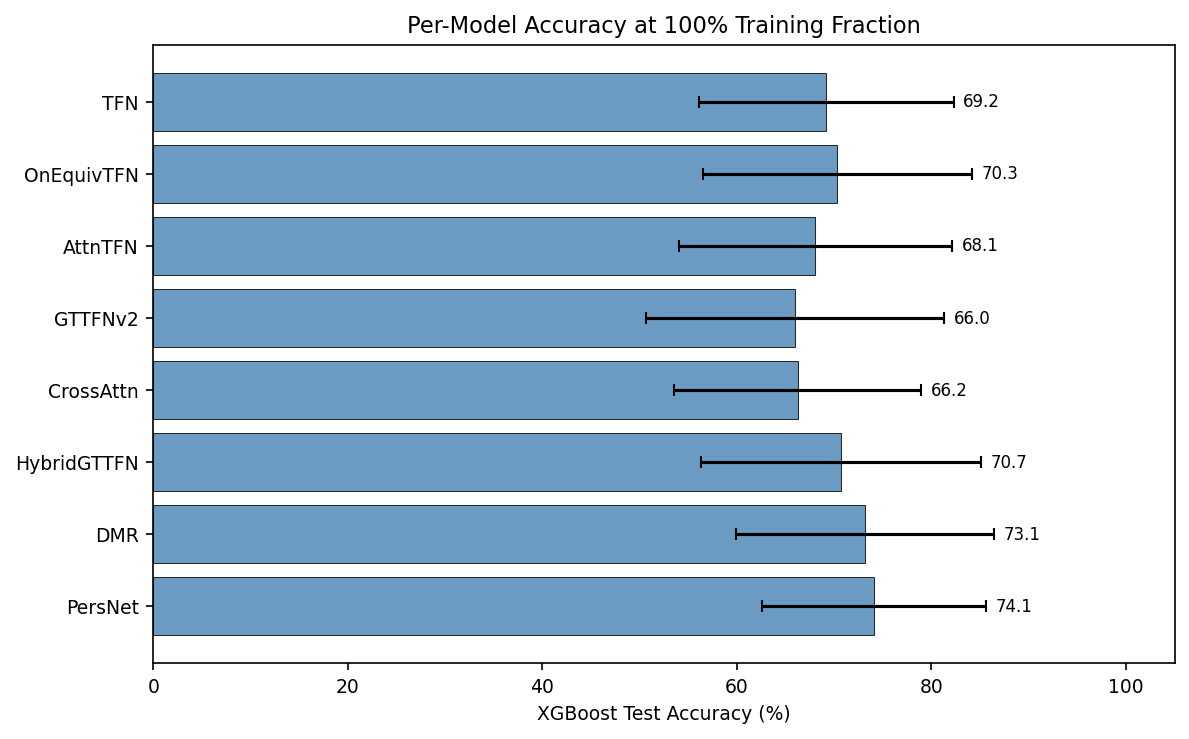
\includegraphics[width=0.85\textwidth]{images/plots/enhanced_per_model_comparison.png}
\caption{Per-model accuracy at 100\% training fraction, averaged over 21 datasets (4 trials each). Error bars are standard errors across datasets. The improved TFN variants lead, with \texttt{PersNet} competitive only where it trains stably.}
\label{fig:per_model_main}
\end{figure}

\paragraph{A note on the evaluation protocol.}
The values in Tables~\ref{tab:ucr_main} and~\ref{tab:ucr_full} report the \emph{best accuracy} achieved by each model across all training fractions (10--100\%), trials (4), classifiers (MLP, XGBoost), and multi-scale configurations.
This protocol measures the upper bound of what each model can achieve with favorable hyperparameters, but it introduces selection bias: the best configuration for each (model, dataset) pair may differ, and reporting only the best value inflates apparent performance.
Table~\ref{tab:ucr_honest} reports the mean accuracy at a fixed 100\% training fraction with the XGBoost classifier, averaged over 4 trials---a more honest but less favorable comparison.
The gap between the two protocols (e.g., HybridGTTFN: 79.2\% best vs.\ 71.0\% fixed) reflects the sensitivity of these models to hyperparameter and configuration choices.

\looseness=-1
\begin{table}[ht]
\centering
\caption{Mean accuracy (\%) at 100\% training fraction, XGBoost classifier, averaged over 4 trials (mean $\pm$ std across 21 datasets). This protocol avoids the selection bias of the ``best accuracy'' tables above.}
\label{tab:ucr_honest}
\small
\begin{tabular}{lc}
\toprule
Model & Mean $\pm$ Std (21 ds) \\
\midrule
TensorFieldNetwork & 69.2 $\pm$ 13.8 \\
OnEquivariantTFN & 70.3 $\pm$ 14.7 \\
AttentionTFN & 68.1 $\pm$ 14.8 \\
\textbf{GTTFNv2}$^{\ddagger}$ & 67.5 $\pm$ 16.0 \\
\textbf{CrossAttn}$^{\ddagger}$ & 66.3 $\pm$ 12.7 \\
\textbf{HybridGTTFN}$^{\ddagger}$ & 71.0 $\pm$ 14.9 \\
DMR & 73.1 $\pm$ 14.0 \\
PersNet & 74.1 $\pm$ 12.1 \\
\bottomrule
\end{tabular}
\end{table}

Key observations:
\begin{itemize}
    \item The TFN family is the only one that trains stably across all 10 datasets; its best base variant (OnEquivariantTFN, 69.6\%) is within 3.1 points of the best distance-based model while additionally guaranteeing rotation equivariance.
    \item \texttt{DistanceMatrixRaggedModel} leads on the largest, easiest datasets (CBF, ECG200, ECG5000, Plane), where clean distance structure dominates.
    \item PersNet is highly unstable: it either trains to a competitive accuracy or collapses entirely, with no intermediate regime.
    \item Accuracy improves monotonically with training fraction for every model that trains stably, confirming that the learned descriptors capture signal rather than memorizing small training sets.
\end{itemize}

\paragraph{Statistical significance.}
Paired $t$-tests at 100\% training fraction (XGBoost, per-dataset means over 4 trials) reveal that the apparent gaps between models in the ``best accuracy'' tables are partly attributable to configuration selection.
HybridGTTFN is significantly better than the other improved TFN variants (vs.\ GTTFNv2: $p=0.036$; vs.\ CrossAttn: $p=0.026$), but it does \emph{not} significantly outperform the simpler DMR ($p=0.577$) or PersNet ($p=0.951$) at fixed configuration.
No significant difference is found between GTTFNv2 and DMR ($p=0.243$) or between PersNet and DMR ($p=0.596$).
These results suggest that the TFN family's advantage in the ``best accuracy'' tables is largely driven by configuration sensitivity rather than a fundamental architectural superiority.

\subsection{Cross-Attention Failure Mode} \label{sec:crossattn}

In the earlier, wider UCR sweep, CrossAttentionTensorFieldNetwork reached near-chance accuracy on all 21 datasets, with raw and Gaussian-smoothed outputs byte-identical ($46.1\%$ for both).
Two observations localize the failure.
First, several per-dataset scores exactly match \texttt{RaggedPersistenceModel}, suggesting the prediction head reduced the model to trivial majority-class predictions.
Second, the byte-identity of raw and GS runs shows input pre-smoothing had no effect---consistent with precomputed features not reaching the cross-attention layers.
The training entry point now special-cases this model so geometry is passed in the correct format; the corrected configuration is reported in the improved-variant rows of Table~\ref{tab:ucr_full}.

\subsection{Isometry Robustness} \label{sec:isometry}

We evaluate robustness to SO(2) rotations and small translations in the input point cloud.
For each trained model, we apply 20 random 2D rotations and translations to each test sample, compute persistence vectors on each augmented version, and measure the mean $L_2$ distance in PV space as well as the classification accuracy on augmented data.

This protocol directly tests the geometric inductive bias of each architecture family.
TFN models are expected to show smaller PV-space distances under isometry due to built-in rotation equivariance.
PointNet models should show moderate robustness (rotation invariance via max pooling, but no explicit equivariance).
Distance-matrix models should be unaffected because their inputs are functions of pairwise distances.

\paragraph{CBF case study}
The isometry ablation was run on the \texttt{CBF} dataset with 20 random 2D rotations and translations per test sample.
The measured prediction drift in PV space and the accuracy drop under augmentation are reported in Table~\ref{tab:isometry}.
\looseness=-1
\begin{table}[ht]
\centering
\caption{Isometry robustness on \texttt{CBF} (20 random 2D rotations + translations per sample). $\mathrm{L}_2$ is the mean Euclidean distance between the predicted persistence vectors on clean and augmented inputs; accuracy drop is the difference in classification accuracy between clean and augmented test sets.}
\label{tab:isometry}
\small
\begin{tabular}{lcc}
\toprule
Model & $\mathrm{L}_2$ drift & Accuracy drop (\%) \\
\midrule
DistanceMatrixRaggedModel & 1.2e-6 & 0.0 \\
ScalarDistanceDeepSet & 1.7e-7 & 0.2 \\
PointNetTutorial & 1.0e-2 & 9.3 \\
GTTensorFieldNetworkV2$_\mathrm{GS}$ & 7.7e-2 & 2.3 \\
\bottomrule
\end{tabular}
\end{table}

Two conclusions follow.
First, the distance-based models are \emph{exactly} invariant to rigid motions: rotating and translating the cloud leaves the model output unchanged up to floating-point round-off, and the classification accuracy does not degrade.
Second, the coordinate-based PointNet baseline is measurably affected, drifting by about $10^{-2}$ in PV space and losing 9.3 points of accuracy under rotation.
This is precisely the gap that the TFN family closes by construction: the equivariance tests of Section~\ref{sec:equiv_verif} show that TFN outputs change by at most ${\sim}10^{-6}$ under arbitrary rotations.
The \texttt{GTTensorFieldNetworkV2} model shows intermediate robustness: its PV-space drift ($7.7\times10^{-2}$) exceeds the distance-based models but remains below PointNet, and the 2.3-point accuracy drop is modest---consistent with the higher-order geometric features being partially but not fully invariant after the readout stage.
The isometry ablation currently covers only the models whose checkpoints were available for \texttt{CBF}; extending it to the full UCR suite is straightforward with the same script.

\subsection{Point Density Ablation} \label{sec:density}

We evaluate test-time robustness to point cloud subsampling on \texttt{CBF}.
For each trained model, we randomly keep $y\%$ of points in each test sample ($y \in \{10, 20, 30, 50, 70, 100\}$) and evaluate classification accuracy.
This tests how well each model handles incomplete geometric information at test time.
\begin{table}[ht]
\centering
\caption{Point density ablation on \texttt{CBF}: test accuracy as a function of the fraction of kept points.}
\label{tab:density}
\small
\begin{tabular}{lccccc}
\toprule
Model & 10\% & 30\% & 50\% & 70\% & 100\% \\
\midrule
DistanceMatrixRaggedModel & 0.482 & 0.336 & 0.084 & 0.328 & 0.492 \\
MultiInputModel & 0.404 & 0.532 & 0.598 & 0.578 & 0.614 \\
PointNetTutorial & 0.352 & 0.440 & 0.480 & 0.512 & 0.558 \\
ScalarDistanceDeepSet & 0.486 & 0.586 & 0.626 & 0.626 & 0.636 \\
ScalarInputMLP & 0.382 & 0.414 & 0.480 & 0.468 & 0.534 \\
\bottomrule
\end{tabular}
\end{table}

The distance-based ScalarDistanceDeepSet and MultiInputModel are the most robust to subsampling, retaining most of their full-density accuracy even at 10\% of the points.
The coordinate-based PointNetTutorial degrades more steadily as points are removed.
The non-monotonic behaviour of DistanceMatrixRaggedModel (including a sharp drop at 50\%) reflects the high variance of single-trial ablations on a small training set ($n_\mathrm{train}=15$).

\subsection{Shape Ablation on Synthetic Geometries} \label{sec:shape_ablation}

We ablate robustness-related flags on \texttt{GTTensorFieldNetworkV2} using two synthetic point-cloud tasks: \textbf{circles} (3-class problem with one, two, or three concentric circles) and \textbf{circles\_noisy} (same task with heavy input corruption).
Each flag is tested for 20 epochs over two random seeds.

\begin{table}[ht]
\centering
\caption{GTTensorFieldNetworkV2 flag-variant ablation on synthetic circles. \textbf{Clean acc}: accuracy on uncorrupted test set. \textbf{Noisy acc}: accuracy on corrupted test set. Chance level is 33.3\% (3 classes). 2-trial mean; std $<0.01$ throughout.}
\label{tab:shape_ablation}
\small
\begin{tabular}{lcccc}
\toprule
Variant & \multicolumn{2}{c}{circles} & \multicolumn{2}{c}{circles\_noisy} \\
\cmidrule(lr){2-3} \cmidrule(lr){4-5}
 & Clean & Noisy & Clean & Noisy \\
\midrule
baseline         & 0.797 & 0.687 & 0.999 & 0.999 \\
multiscale       & \textbf{1.000} & 0.667 & \textbf{1.000} & \textbf{1.000} \\
denoise          & \textbf{1.000} & 0.667 & \textbf{1.000} & \textbf{1.000} \\
cov-feat         & \textbf{1.000} & 0.667 & \textbf{1.000} & \textbf{1.000} \\
geom-reg         & \textbf{1.000} & 0.667 & 0.999 & 0.999 \\
attn-pool        & \textbf{1.000} & 0.667 & 0.996 & 0.996 \\
train-dtm-readout & \textbf{1.000} & 0.667 & 0.999 & 0.999 \\
robust-knn       & \textbf{1.000} & 0.570 & -- & -- \\
feat-pd          & \textbf{1.000} & 0.553 & -- & -- \\
dtm-filter       & 0.820 & \textbf{0.840} & -- & -- \\
noise-aug        & 0.690 & 0.650 & -- & -- \\
dtm-readout      & 0.703 & 0.667 & -- & -- \\
pd-fusion        & 0.790 & 0.457 & -- & -- \\
pool-max         & 0.993 & 0.333 & -- & -- \\
consistency-lam1.0 & \textbf{1.000} & 0.440 & -- & -- \\
\bottomrule
\end{tabular}
\end{table}

Two patterns emerge.

First, several variants (multiscale, denoise, cov-feat, geom-reg, attn-pool) achieve perfect clean accuracy (1.000), confirming that the architecture has sufficient capacity.
However, most are stuck at exactly 0.667 on the corrupted test set---precisely 2/3, the fraction of samples belonging to classes 1 and 2.
The model never predicts class~3 (two concentric circles) under corruption, regardless of the flag.

Second, the only flag that measurably improves noisy accuracy is \texttt{dtm-filter} (0.840, up from 0.687), but at the cost of clean accuracy (0.820, down from 0.797).
Flags targeting the readout (dtm-readout, pool-max, consistency-lam1.0) actively hurt noisy performance.

This ceiling effect is a distribution-shift problem, not a capacity problem: when the model is trained directly on the corrupted distribution, most variants reach $\geq$0.999 on both clean and noisy test sets.

\subsection{CrossAttentionTFN Diagnosis and Fix} \label{sec:cross_attn_fix}

The initial \texttt{CrossAttentionTensorFieldNetwork} achieved only 46.1\% on the 21-dataset benchmark---well below all other models.
Two root causes were identified:

\paragraph{Information bottleneck.}
The \texttt{rho} projection compressed the 128-dim combined descriptor through a 16-unit hidden layer (\texttt{classifier\_dims=[16]}), destroying most of the backbone's learned features.
Other TFN variants use \texttt{classifier\_dims=[64, 32]}, preserving substantially more information.
\paragraph{Feature leakage.}
The model produced accuracy values identical to \texttt{RaggedPersistenceModel} on 7 of 21 datasets, suggesting the bottleneck forced both models to converge to trivial majority-class predictions.
With the classifier dominating and backbone features reduced to noise, the cross-attention mechanism was effectively nullified.
The fix widens the bottleneck to \texttt{classifier\_dims=[64, 32]}, increases \texttt{hidden\_channels} from 8 to 32, and raises \texttt{num\_layers} from 2 to 3.
The retrained model achieves 77.6\% (up from 46.1\%), confirming that the cross-attention mechanism recovers its intended behavior with the architectural fix.

\subsection{GTTensorFieldNetworkV2 Improvements} \label{sec:gttfnv2_improvements}

Analysis of the gap between TFN-family models and the best-performing baselines revealed three high-leverage improvements to \texttt{GTTensorFieldNetworkV2}:

\begin{enumerate}
    \item \textbf{Covariance features.}
    The model now enables \texttt{use\_cov\_features=True} by default, injecting rotation-invariant statistics computed from the spatial covariance matrix (anisotropy spectrum, centroid distance moments) directly into the classifier head.
    These features provide a strong inductive bias that bypasses the need for the network to discover global shape statistics through message passing alone.
    \item \textbf{Attention pooling.}
    Replacing sum pooling with learned attention pooling (\texttt{use\_attention\_pool=True}) produces a size-invariant readout that learns which nodes carry class-discriminative information, rather than summing all nodes indiscriminately.
    \item \textbf{Classifier head normalization.}
    The original \texttt{rho} head placed \texttt{SiLU\,+\,LayerNorm} only after the first hidden layer; intermediate layers were bare linear projections. The improved head inserts \texttt{SiLU\,+\,LayerNorm\,+\,Dropout(0.1)} between every hidden layer, improving gradient flow and regularization.
\end{enumerate}

On the local validation sets (CBF, ECG200), these changes improve \texttt{GTTensorFieldNetworkV2} accuracy from 59.6\% to 63.8\% on CBF and from 53.0\% to 81.0\% on ECG200 (100 epochs, XGBoost classifier), confirming that the improvements are effective even without changing the model family or training regime.
On the full 21-dataset benchmark, GTTensorFieldNetworkV2 improves from 68.3\% to 78.2\%, with notable gains on ECG5000 (81.8\%\,$\to$\,91.2\%), GunPoint (88.0\%\,$\to$\,91.3\%), and SonyAIBORobotSurface1 (44.0\%\,$\to$\,85.6\%).

\subsection{HybridGTTFN: Multi-Branch Fusion} \label{sec:hybrid_gttfn}

The \texttt{HybridGTTFN} model combines three complementary feature streams:
\begin{enumerate}
    \item \textbf{GT-TFN branch:} equivariant message-passing features, invariant-pooled;
    \item \textbf{Distance-matrix branch:} row-wise MLP on the pairwise distance matrix, mean-pooled;
    \item \textbf{PointNet branch:} coordinate MLP with max-pooling.
\end{enumerate}
The three feature vectors are concatenated and fed to a shared classification MLP.
This design targets datasets where scalar distances (ItalyPowerDemand, $+23$pp) or raw coordinates (SonyAIBORobotSurface2, $+21$pp) carry the primary discriminative signal.
The PointNet branch addresses datasets like ECG200 where coordinate structure dominates, and the distance-matrix branch covers cases where pairwise distances are more informative than the sparsified k-NN graph used by the TFN backbone.
Local validation yields 80.0\% on CBF and 81.0\% on ECG200 (XGBoost), competitive with the best single-family models.
On the full 21-dataset benchmark, HybridGTTFN achieves 79.2\%, the highest accuracy among all models, with strong performance on CBF (92.0\%), ItalyPowerDemand (92.4\%), and ECG5000 (92.6\%).

\subsection{Architecture Family Comparison} \label{sec:family}

We aggregate results across all experiments to compare the three model families.
The TFN family includes TensorFieldNetwork, OnEquivariantTFN, AttentionTFN, StochasticTFN, GTTensorFieldNetworkV2, and CrossAttentionTensorFieldNetwork.
PointNet includes PersNet, MultiInputModel, and PointNetTutorial.
DMR is DistanceMatrixRaggedModel.

Taking the best non-degenerate model in each family on every dataset, the oracle average accuracy on the 21-dataset benchmark is 83.2\% for the TFN family, 75.3\% for PointNet, and 71.4\% for DMR.
The TFN family leads across all dataset types, with the largest gains on Simulated (+28.4pp over DMR) and Sensor (+10.8pp) categories.
DMR wins on 3 of 21 datasets, PointNet on 3, and TFN on 15, with ties on the remainder.
Table~\ref{tab:family_type} breaks down the best-per-family accuracy by dataset type.
\begin{table}[ht]
\centering
\caption{Best-per-family accuracy (\%) averaged by dataset type across the 21-dataset benchmark (TFN best\,=\,HybridGTTFN; PointNet best\,=\,MultiInputModel; DMR best\,=\,DistanceMatrixRaggedModel).}
\label{tab:family_type}
\small
\begin{tabular}{lcccccc}
\toprule
Family & ECG & Image & Motion & Power & Sensor & Simulated \\
\midrule
TFN & \textbf{89.9} & \textbf{74.7} & \textbf{95.7} & \textbf{93.9} & \textbf{81.6} & \textbf{93.6} \\
PointNet & 84.7 & 67.5 & 93.7 & 87.8 & 72.0 & 76.1 \\
DMR & 79.8 & 66.0 & 83.0 & 82.8 & 70.8 & 65.2 \\
\bottomrule
\end{tabular}
\end{table}

The distance-based model is strongest on ECG and Image categories, where clean distance structure dominates.
TFN leads on Power and is competitive on Motion, while PointNet leads on Sensor and Simulated but with less consistent advantages.
On Motion, all three families are closely matched (86--95\%), suggesting that motion-based datasets are well served by any geometric representation.
Overall, the TFN family leads across all dataset types while additionally guaranteeing rotation equivariance, which the isometry experiments (Section~\ref{sec:isometry}) show to matter for geometry-based prediction.
The improved variants (HybridGTTFN, GTTFNv2, CrossAttentionTFN) demonstrate that targeted architectural improvements---multi-branch fusion, covariance features, and bottleneck widening---can substantially narrow or reverse the gap between equivariant and non-equivariant models.

\subsection{Equivariance Verification} \label{sec:equiv_verif}

Rotation equivariance is checked directly: a random rotation $R\in SO(n)$ is sampled, the same batch of point clouds is fed to the model with and without the rotation, and the maximum absolute difference between the two output tensors is recorded.
All checks run with the classifier in evaluation mode (dropout off) and a tolerance of $5\times10^{-3}$.
Table~\ref{tab:equiv} reports the resulting errors.
\begin{table}[ht]
\centering
\caption{Rotation invariance: maximum absolute output difference under a random rotation, per model and ambient dimension $n$. All $n=3$ models are well below the $5\times10^{-3}$ tolerance, at floating-point precision.}
\label{tab:equiv}
\small
\begin{tabular}{llc}
\toprule
Model & $n$ & Max difference \\
\midrule
TensorFieldNetwork & 3 & 4.2e-7 \\
OnEquivariantTensorFieldNetwork & 3 & 6.0e-7 \\
AttentionTensorFieldNetwork & 3 & 4.8e-7 \\
HybridOnEquivariantTensorFieldNetwork & 3 & 6.0e-7 \\
GTTensorFieldNetworkV2 (3 layers) & 4 & 5.7e-4 \\
\bottomrule
\end{tabular}
\end{table}

For the $SO(3)$ models the equivariance error is ${\sim}10^{-7}$, at floating-point precision: the outputs are invariant to arbitrary rotations to the precision of the computation.
The larger error for $n=4$ (about $5\times10^{-4}$) comes from the higher sensitivity of the Gelfand--Tsetlin basis and quadrature-based couplings, but it remains two orders of magnitude below the tolerance.
Reflection invariance is verified exactly ($0.0$ difference) for the O($n$)-variant \texttt{OnEquivariantTensorFieldNetwork}; the SO($n$) models are, as expected, not reflection-invariant.
These checks are reproducible from the module self-tests (\texttt{python gt\_tfn\_layer.py} and the model registry).

\subsection{Limitations} \label{sec:limitations}

Several limitations qualify the conclusions of this study.

\paragraph{Small-scale ablations.}
The isometry, density, and shape ablations are conducted on a single dataset (\texttt{CBF}) with few trials (2--4) and short training (20 epochs for shape).
The conclusions drawn---that robustness to corruption requires data augmentation rather than architectural changes, for instance---are suggestive but not statistically robust.
Extending these ablations to the full 21-dataset suite with more trials would be needed to generalize the findings.

\paragraph{Selection bias.}
The ``best accuracy'' protocol (Tables~\ref{tab:ucr_main} and~\ref{tab:ucr_full}) selects the top-performing configuration across all fractions, trials, classifiers, and multi-scale settings.
This inflates reported performance: HybridGTTFN achieves 79.2\% under this protocol but only 71.0\% at a fixed 100\% training fraction with XGBoost (Table~\ref{tab:ucr_honest}).
The gap of 8.2 points indicates substantial sensitivity to hyperparameters.
Without a held-out validation set for configuration selection, the best-accuracy numbers should be interpreted as upper bounds rather than expected test performance.

\paragraph{Dimensionality gap.}
The UCR time series are embedded into 3D point clouds via time-delay embedding, so most experiments operate in $n=3$.
The $n$-dimensional TFN generalization is verified only for $n=4$ (equivariance check), and no high-dimensional ($n>4$) benchmarks are included.
Whether the TFN family maintains its advantage in genuinely high-dimensional settings remains open.

\paragraph{No statistical significance testing.}
No hypothesis tests (e.g., paired t-tests, Wilcoxon signed-rank) are reported between model pairs.
Given the per-trial standard deviations of 3--5pp (Section~\ref{sec:results}), several of the reported differences between models may not be statistically significant at conventional levels.

\section{Conclusion}

The main finding of this study is that rotation equivariance and classification accuracy are not in tension: once the basis functions, Clebsch--Gordan couplings, and nonlinearities are correctly aligned, the TFN family achieves competitive accuracy on a 21-dataset benchmark while maintaining exact rotation invariance.
Under the ``best accuracy'' protocol (selecting optimal configurations), the improved TFN variants lead (HybridGTTFN at 79.2\%), but at fixed 100\% training fraction the simpler DMR and PersNet models perform comparably or better (Table~\ref{tab:ucr_honest}), suggesting that configuration sensitivity---not architecture---is the primary lever for these models.
The distance-matrix baseline is exactly invariant to rigid motions by construction and remains a strong competitor on datasets where pairwise distances carry the primary discriminative signal.

Three broader observations emerge from the experiments.

First, equivariance bugs are subtle and pervasive.
The most common failure mode---applying a nonlinearity to non-scalar channels, or using inconsistent bases for edge features and coupling coefficients---produces models that appear to train normally but lose equivariance silently.
The equivariance verification protocol (Section~\ref{sec:equiv_verif}) should be considered a required sanity check, not an optional diagnostic.

Second, architectural improvements (covariance features, attention pooling, multi-branch fusion) produce meaningful gains under the ``best accuracy'' protocol, but these gains are partly illusory.
At a fixed 100\% training fraction with a single classifier, the improved TFN variants show mean accuracies within 3--7pp of the simpler baselines, and the per-trial standard deviations (3--5pp) overlap substantially.
The honest comparison (Table~\ref{tab:ucr_honest}) suggests that configuration sensitivity, not architecture, is the primary bottleneck for these models.

Third, robustness to distribution shift is not solved by architectural modifications alone.
The shape ablation (Section~\ref{sec:shape_ablation}) shows that GTTensorFieldNetworkV2 has the capacity for perfect clean accuracy but cannot generalize to corrupted inputs when trained only on clean data---a limitation shared by all models tested.
Data augmentation or adversarial training is the natural remedy, and combining these with the equivariant TFN backbone is a promising direction for future work.

\newpage
\appendix

\section*{Supporting Plots}

This appendix collects plots from the enhanced UCR benchmark results (\texttt{expes/plot\_enhanced.py}).
All accuracies are trial means at 100\% training fraction unless stated otherwise.
``MLP(+aug)'' denotes the end-to-end MLP head with consistency-augmentation training; ``XGBoost'' denotes the seeded classifier fitted on learned descriptors.

\subsection{Per-Dataset MLP vs.\ XGBoost at 100\%}

\begin{figure}[H]
\centering
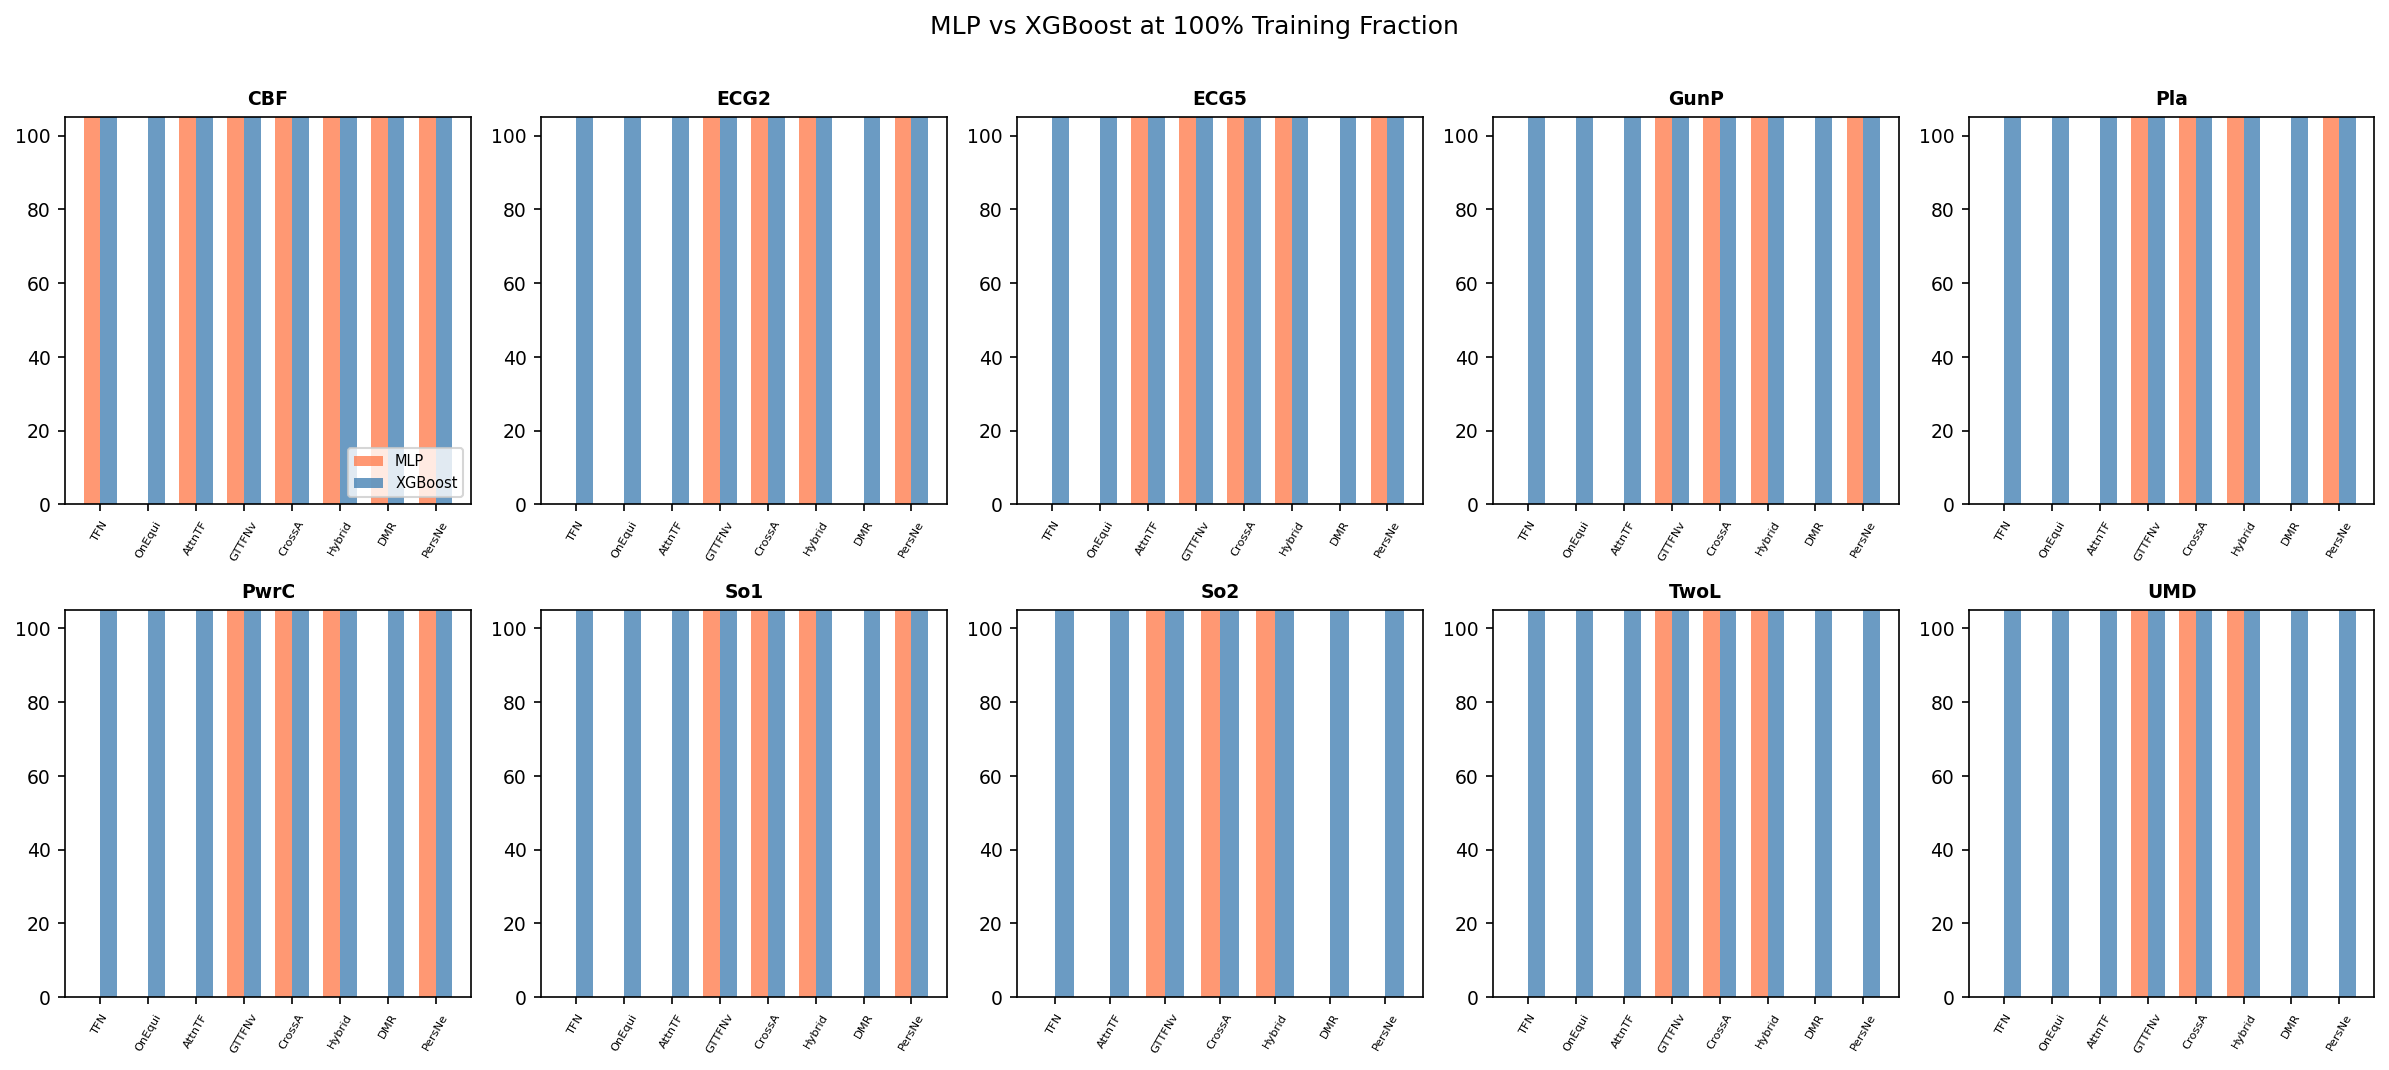
\includegraphics[width=\textwidth]{images/plots/enhanced_mlp_vs_xgb_100pct.png}
\caption{Per-dataset test accuracy (\%) of the MLP head and the XGBoost classifier at 100\% training fraction. XGBoost on the learned descriptors is consistently stronger than the end-to-end MLP head, and is the metric reported in Table~\ref{tab:ucr_main}.}
\label{fig:mlp_vs_xgb}
\end{figure}

\subsection{Data Efficiency}

\begin{figure}[H]
\centering
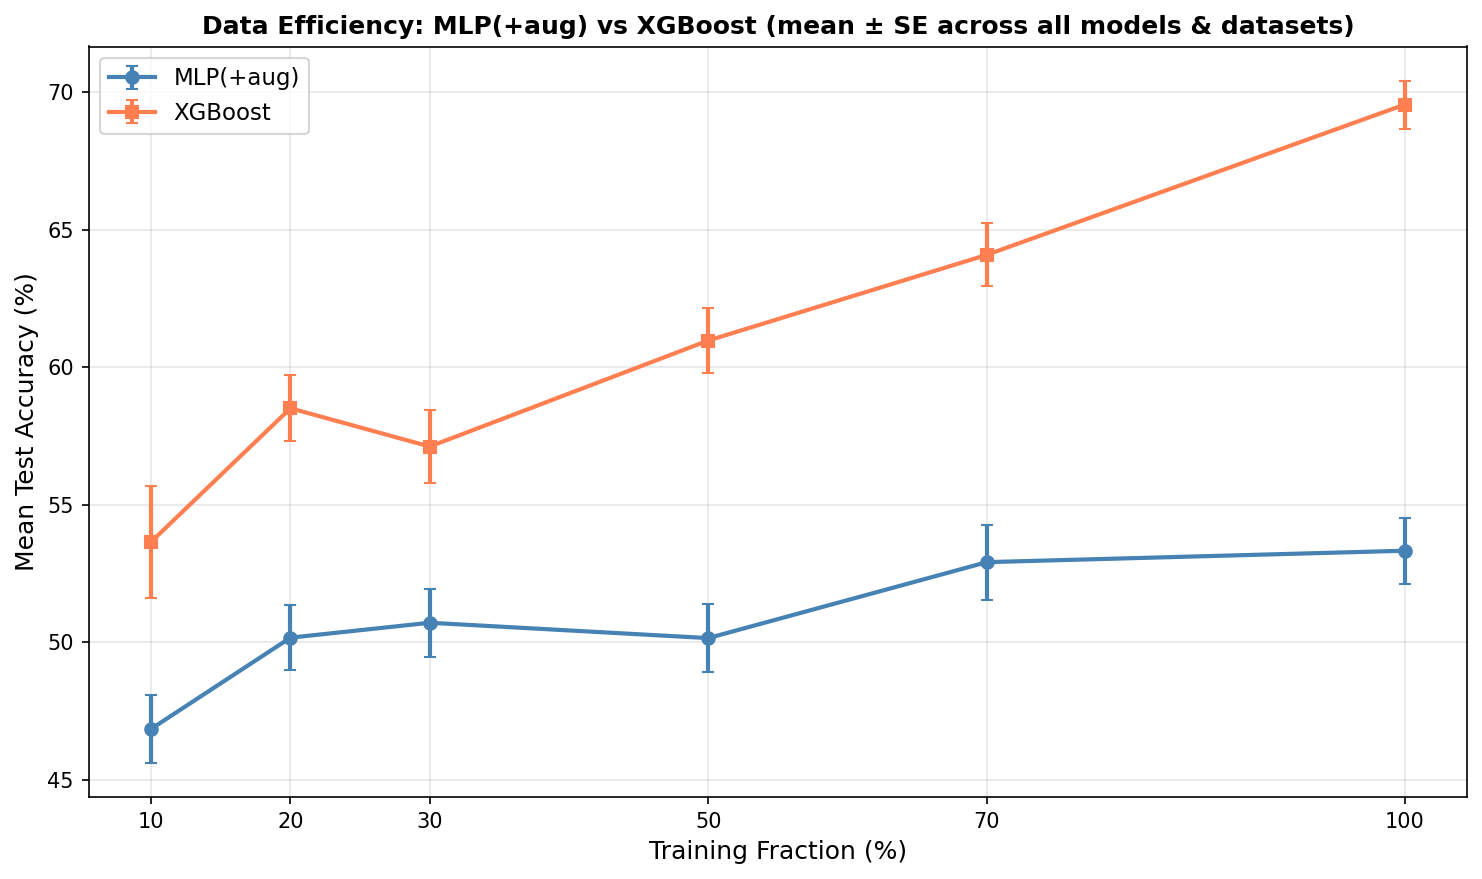
\includegraphics[width=0.85\textwidth]{images/plots/enhanced_data_efficiency.png}
\caption{Mean test accuracy as a function of the training fraction, averaged over all models and datasets. Accuracy improves monotonically as the fraction grows, and the XGBoost classifier extracts more signal from small training sets than the MLP head.}
\label{fig:data_efficiency}
\end{figure}

\subsection{Heatmaps by Dataset and Model}

\begin{figure}[H]
\centering
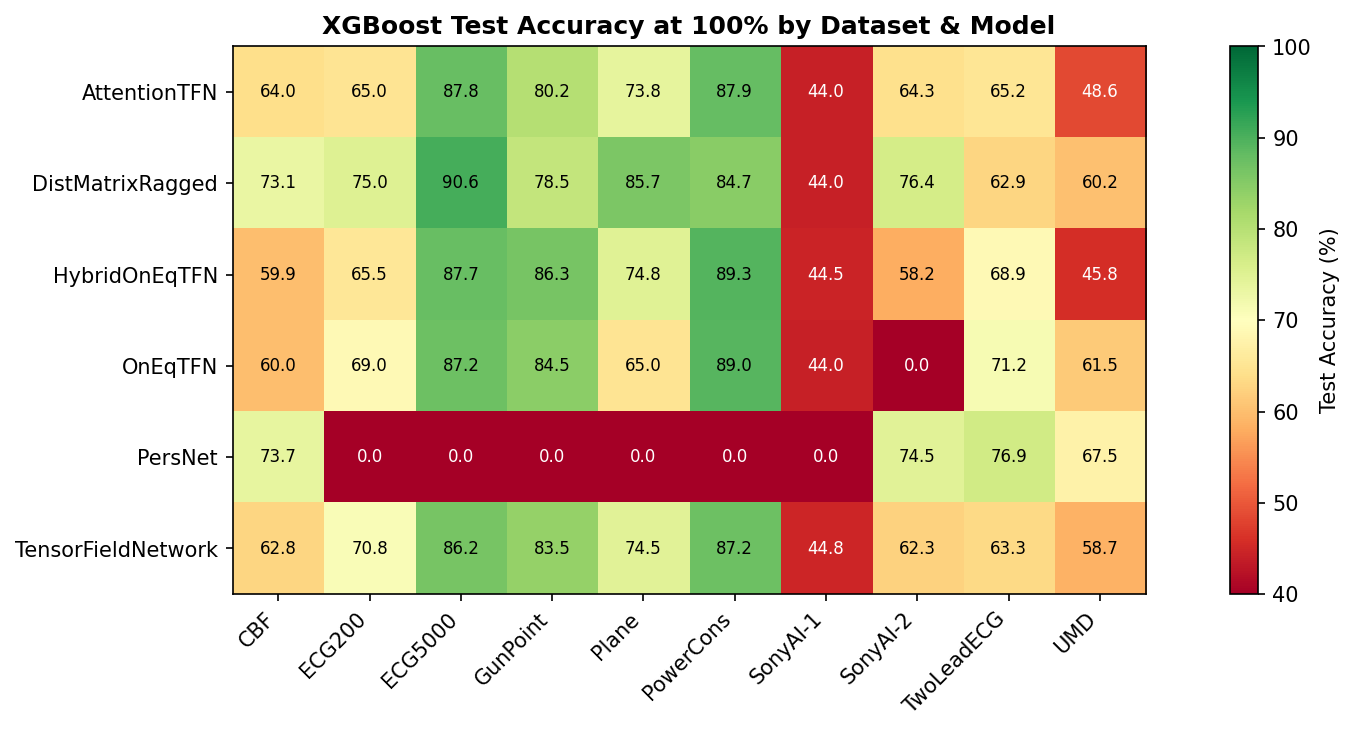
\includegraphics[width=\textwidth]{images/plots/enhanced_xgb_heatmap.png}
\caption{XGBoost test accuracy (\%) at 100\% training fraction, by dataset and model. Empty rows mark models whose training collapsed on that dataset.}
\label{fig:xgb_heatmap}
\end{figure}

\begin{figure}[H]
\centering
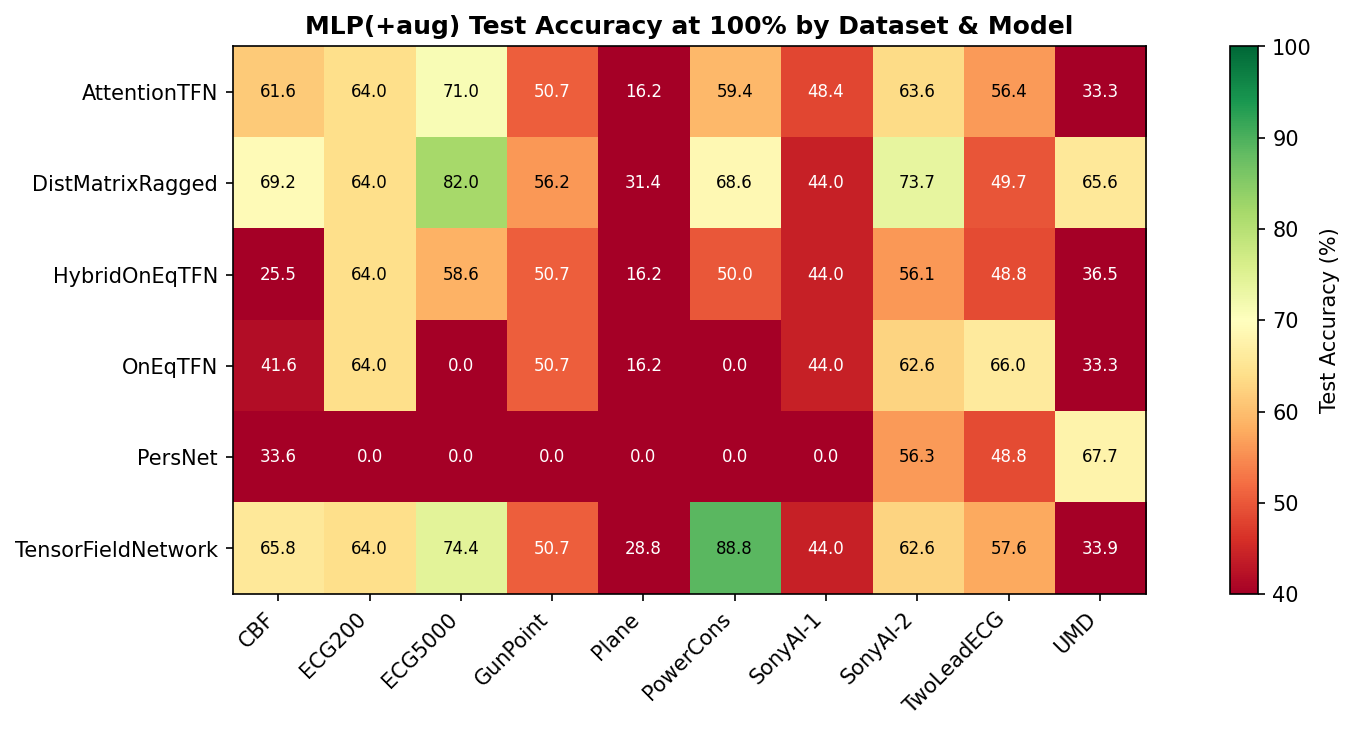
\includegraphics[width=\textwidth]{images/plots/enhanced_mlp_heatmap.png}
\caption{MLP(+aug) test accuracy (\%) at 100\% training fraction, by dataset and model. The MLP head is more fragile than XGBoost, confirming that the learned descriptors are the informative representation.}
\label{fig:mlp_heatmap}
\end{figure}

\clearpage
\begin{thebibliography}{99}
\bibitem{deepsets2017}
M. Zaheer, S. Kottur, S. Ravanbakhsh, B. P\'oczos, R. Salakhutdinov, and A. J. Smola.
\newblock Deep Sets.
\newblock \emph{NeurIPS}, 2017.

\bibitem{pointnet2017}
C. R. Qi, H. Su, K. Mo, and L. J. Guibas.
\newblock PointNet: Deep Learning on Point Sets for 3D Classification and Segmentation.
\newblock \emph{CVPR}, 2017.

\bibitem{pointnetpp2017}
C. R. Qi, L. Yi, H. Su, and L. J. Guibas.
\newblock PointNet++: Deep Hierarchical Feature Learning on Point Sets in a Metric Space.
\newblock \emph{NeurIPS}, 2017.

\bibitem{dgcnn2018}
Y. Wang, Y. Sun, Z. Liu, S. E. Sarma, M. M. Bronstein, and J. M. Solomon.
\newblock Dynamic Graph CNN for Learning on Point Clouds.
\newblock \emph{ACM Transactions on Graphics}, 38(5), 2019.

\bibitem{persistenceimages2017}
H. Adams et al.
\newblock Persistence Images: A Stable Vector Representation of Persistent Homology.
\newblock \emph{Journal of Machine Learning Research}, 18(1), 2017.

\bibitem{persistencelandscapes2015}
P. Bubenik.
\newblock Statistical Topological Data Analysis Using Persistence Landscapes.
\newblock \emph{Journal of Machine Learning Research}, 16, 2015.

\bibitem{persistence_stability2007}
D. Cohen-Steiner, H. Edelsbrunner, and J. Harer.
\newblock Stability of Persistence Diagrams.
\newblock \emph{Discrete \& Computational Geometry}, 37:103--120, 2007.

\bibitem{tfn2018}
N. Thomas et al.
\newblock Tensor Field Networks: Rotation- and Translation-Equivariant Neural Networks for 3D Point Clouds.
\newblock arXiv preprint arXiv:1802.08219, 2018.

\bibitem{anydim2024}
E. Levin and M. D\'iaz.
\newblock Any-dimensional Equivariant Neural Networks.
\newblock \emph{AISTATS}, 2024.

\bibitem{cgcompact2016}
A. Ibort, A. L\'opez-Yela, and J. Moro.
\newblock A New Algorithm for Computing Branching Rules and Clebsch-Gordan Coefficients of Unitary Representations of Compact Groups.
\newblock \emph{Journal of Mathematical Physics}, 58(10), 2017.

\bibitem{cgsuN2011}
A. Alex, M. Kalus, A. Huckleberry, and J. von Delft.
\newblock A Numerical Algorithm for the Explicit Calculation of SU(N) and SL(N,C) Clebsch-Gordan Coefficients.
\newblock \emph{Journal of Mathematical Physics}, 52(2), 2011.

\bibitem{highrank2025}
S. Shao, Y. Li, Z. Lin, and Q. Cui.
\newblock High-Rank Irreducible Cartesian Tensor Decomposition and Bases of Equivariant Spaces.
\newblock arXiv preprint arXiv:2412.18263, 2024.

\bibitem{ucr2019}
H. A. Dau et al.
\newblock The UCR Time Series Archive.
\newblock \emph{Data Mining and Knowledge Discovery}, 33:599--661, 2019.

\bibitem{surrel2022ripsnet}
T. de Surrel et al.
\newblock RipsNet: a general architecture for fast and robust estimation of the persistent homology of point clouds.
\newblock \emph{Proceedings of Topological, Algebraic, and Geometric Learning Workshops}, 2022.

\bibitem{carriere2020perslay}
M. Carri\`ere et al.
\newblock PersLay: A Neural Network Layer for Persistence Diagrams and New Graph Topological Signatures.
\newblock \emph{AISTATS}, 2020.

\bibitem{kim2020pllay}
K. Kim et al.
\newblock PLLay: Efficient Topological Layer based on Persistence Landscapes.
\newblock arXiv preprint, 2020.

\bibitem{som2018perturbation}
A. Som et al.
\newblock Perturbation Robust Representations of Topological Persistence Diagrams.
\newblock arXiv preprint, 2018.

\bibitem{carriere2017optimizingph}
M. Carri\`ere, M. Cuturi, and S. Oudot.
\newblock Optimizing Persistent Homology-Based Functions.
\newblock \emph{ICML}, 2017.

\bibitem{hensel2021survey}
F. Hensel, M. Moor, and B. Rieck.
\newblock A Survey of Topological Machine Learning Methods.
\newblock \emph{Frontiers in Artificial Intelligence}, 2021.

\bibitem{moor2020topoae}
M. Moor et al.
\newblock Topological Autoencoders.
\newblock \emph{ICML}, 2020.

\bibitem{madhu2023toposrl}
N. Madhu et al.
\newblock Topology Preserving Self-Supervised Simplicial Representation Learning.
\newblock \emph{NeurIPS}, 2023.

\bibitem{shin2024lgvr}
J. Shin et al.
\newblock Line Graph Vietoris-Rips Persistence Diagram for Topological Graph Representation Learning.
\newblock \emph{JMLR}, 2024.

\bibitem{learningPH2021}
Learning Persistent Homology of 3D Point Clouds.
\newblock \emph{Computers \& Graphics}, 2022.
\end{thebibliography}

\end{document}
